\documentclass[a4paper,12pt]{article}

\usepackage{amsmath,amssymb,amsthm,multicol,tikz,enumitem}
\usepackage{hyperref}
\usepackage{fancyvrb}
\usepackage[margin=2cm]{geometry}
\usetikzlibrary{calc,arrows.meta}

\newcommand\N{\mathbf{N}}
\newcommand\Q{\mathbf{Q}}
\newcommand\R{\mathbf{R}}
\newcommand\Z{\mathbf{Z}}

\def\ojoin{\setbox0=\hbox{$\bowtie$}%
  \rule[-.02ex]{.25em}{.4pt}\llap{\rule[\ht0]{.25em}{.4pt}}}
\def\leftouterjoin{\mathbin{\ojoin\mkern-5.8mu\bowtie}}
\def\rightouterjoin{\mathbin{\bowtie\mkern-5.8mu\ojoin}}
\def\fullouterjoin{\mathbin{\ojoin\mkern-5.8mu\bowtie\mkern-5.8mu\ojoin}}

\pagestyle{empty}


%\newcommand\answer[1]{}
%\newcommand\ans[1]{}
\newcommand\answer[1]{\\[5pt]{\color{blue}{#1}}\hfill{\color{blue}$\qed$}\\[-5pt]} 
\newcommand\ans[1]{{\color{blue}{#1}}}


\newcommand\rem{\textup{rem}}

\begin{document}

\begin{center}
\parbox{3cm}{\flushleft\bf Discrete\linebreak Structures}
\hfill
\parbox{7cm}{\centering {\bf\Huge Exam, Part 1}}
\hfill
\parbox{3cm}{\flushright\bf Spring 2021 \linebreak May 24}
\end{center}

\hrule\vspace{2pt}\hrule

\hrule


\vspace{5pt}
\begin{enumerate}
\item
% 1.(c)
%Build a DNF or a CNF for a given truth table.
In the Venn diagram each oval represents the area 
where statements $p$, $q$, and $r$ are true
(outside their respective ovals they are false). 
Regions where $f(p,q,r)=\mathtt{True}$ are shaded.
\begin{center}
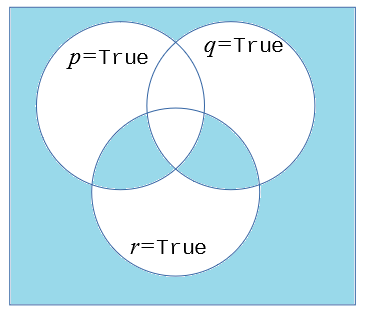
\includegraphics[width=2in]{figs/part1-venn-diagram.png}
\end{center}

\begin{enumerate}
\item 
Create a truth table for this Boolean function $f(p,q,r)$. 
\answer{

\begin{tabular}{|c|c|c||c|}
$p$ & $q$ & $r$ & $f(p,q,r)$ \\ \hline
{\tt False} & {\tt False} & {\tt False} & {\tt True} \\ 
{\tt False} & {\tt False} & {\tt True} & {\tt False} \\
{\tt False} & {\tt True} & {\tt False} & {\tt False} \\
{\tt False} & {\tt True} & {\tt True} & {\tt True} \\
{\tt True} & {\tt False} & {\tt False} & {\tt False} \\
{\tt True} & {\tt False} & {\tt True} & {\tt True} \\
{\tt True} & {\tt True} & {\tt False} & {\tt False} \\
{\tt True} & {\tt True} & {\tt True} & {\tt False} \\
\end{tabular}

Region outside of all ovals is shaded, so $f(\mathtt{False}, \mathtt{False}, \mathtt{False}) = \mathtt{True}$
(1st line in the truth table);
also two more regions are shaded, where just two of the variables are {\tt True}. 
}
\item Create either a Disjunctive Normal Form (DNF) or a Conjunctive Normal Form (CNF) for this function $f(p,q,r)$.\\
{\em Note.} You can pick either a DNF or a CNF \textendash{} whatever
you like; there is no need to construct both.
\answer{

In our situation the DNF would be shorter \textendash{} it is a disjunction of just $3$ conjunctions
(each conjunction describes one row where the Boolean function is {\tt True}). 

\[ f(p,q,r) = (\neg p \wedge \neg q \wedge \neg r) \vee (\neg p \wedge q \wedge r) \vee (p \wedge \neg q \wedge r). \]

(CNF would be a conjunction of $5$ expressions \textendash{} one per every row in the table where the
function is {\tt False}.)
}
\end{enumerate}



\item 
% 2.(b)
% Express an English sentence as a predicate logic expression.
Let $H$ be the set of all humans. We define the following predicates:\\
$K(a,b)$ is true iff when the human $a \in H$ knows a human $b \in H$.\\
$R(a)$ is true iff the human $a$ has travelled from Riga to Frankfurt by train.

Express the following English sentences using the predicates and quantifiers: 
\begin{enumerate}
\item For any two humans $a$ and $b$, person $a$ knows person $b$ iff person $b$ knows person $a$. 
\answer{

\[ \forall a \in H\ \forall b \in H\ (K(a,b) \leftrightarrow K(b,a)). \]
This condition tells that the predicate $K(a,b)$ (which is also a relation of ``knowing'' between two humans) 
is {\em symmetric}. It is also possible to express this as one-way implication.
\[ \forall a \in H\ \forall b \in H\ (K(a,b) \rightarrow K(b,a)). \]

The 2nd expression tells the same thing (you can get the reverse implication, if you switch variables $a$ and $b$). 
So both answers are fine; the 1st answer reflects the English sentence better.
}
\item Not every human knows someone who has travelled from Riga to Frankfurt by train. 
\answer{

\[ \neg \forall a \in H\ \exists b \in H\ (K(a,b) \wedge R(b)). \]
Literally: It is not the case that for any human $a \in H$ there exist a human $b \in H$ such that $a$ knows $b$ and 
$b$ has traveled to Frankfurt. 

If you wish, you can also rewrite this using De Morgan's laws: 
\[ \exists a \in H\ \forall b \in H\ (\neg K(a,b) \vee \neg R(b)). \]
Literally: There is a human $a \in H$ such that for any human $b \in H$ \textendash{} either $a$ does not know $b$ or $b$ did not 
travel from Riga to Frankfurt by train.
}
\end{enumerate}



\item 
% 2.(d)
% Write the negation for a predicate expression; simplify using De Morgan’s laws.
Let $H$ be the set of all humans and the predicates $K(a,b)$ and $R(a)$ are the
same as in the previous exercise. 
Rewrite the statement so that negations are applied only to the predicates directly.
\[ \neg \bigg( \forall a \in H\ \exists b \in H\ \exists c \in H\ \Big( R(a)\ \vee\  \big(K(a,b) \wedge K(a,c) \wedge b \neq c \wedge R(b) \wedge R(c)\big) \Big) \bigg). \]
\answer{

Here we negate the sentence that every human $a \in H$ either himself/herself traveled to Frankfurt or 
he knows two other people $b$ and $c$ (not equal between themselves: $b \neq c$) such that both of them traveled to Frankfurt. 

\[ \bigg( \exists a \in H\ \forall b \in H\ \forall c \in H\ \Big( \neg R(a)\ \wedge\  \big(\neg K(a,b) \vee \neg K(a,c) \vee b = c \vee \neg R(b) \vee \neg R(c)\big) \Big) \bigg). \]
Literally: Some human $a$ is such that s/he did not travel to Frankfurt and also for any other two humans $b,c$, either $a$ does not know at least one
of them, or $b$ is equal to $c$ or at least one among $b$ and $c$ did not travel to Frankfurt.
}






\item 
%3.(a)
% Given a function, prove/disprove that it is injective, surjective or bijective.
Let $f(x) = x^3 + 1$ be a function $f:\R \rightarrow \R$ with real arguments and real values. 
\begin{enumerate}
\item Is $f$ an injective function?
\answer{

Yes, $f$ is an injective function. The easiest way to see it is to notice that $f(x) = x^3 + 1$ is 
strictly monotone (growing) function as a cubic parabola: whenever $x_1 < x_2$ we should also have $f(x_1) < f(x_2)$. 

So it is impossible that some different values $x_1 \neq x_2$ would have equal values $f(x_1) = f(x_2)$, 
since one of the $x_1,x_2$ would be smaller than the other (and we apply the monotonicity). 
}
\item Is $f$ a surjective function?
\answer{

Yes, $f$ is a surjection, since for every $a \in \R$ we can solve the equation: 
\[ x^3 + 1 = a. \]
The root is $x = \sqrt[3]{a - 1}$. If we compute $f(x)$ for this argument we will get the value $a$ we need.
}
\end{enumerate}

\item 
%3.(f)
% Given a binary relation determine if it is reflexive, symmetric, antisymmetric or transitive.
Let $S = \{ 1,2,4,5,7,8 \}$ be the set of all digits not divisible by $3$. 
Define a relation $R \subseteq S^2$: 
\[ R = \left\{ (a,b) \in S^2\ \;\mid\;\ |a-b| \leq 1 \right\}. \]
\begin{enumerate}
\item Is the relation $R$ reflexive? Is it symmetric? Is it transitive?
\answer{

The condition tells that the distance between $a$ and $b$ is no more than $1$. 
So the only pairs in the relation are $R(1,1)$, $R(1,2)$, $R(2,1)$, $R(2,2)$ (and similarly for $4$ and $5$ and also for $7$ and $8$):
Two digits are in this relation if they are the same ($|a - b| = 0$) or they are next to each other. 

Clearly, this relation is reflexive (as $|a - a| = 0$); it is symmetric (since $|a - b| = |b - a|$). 
It is also transitive (because the digits fall into three groups of neighbors \textendash{} if $a$ and $b$ are in the same group
and also $b$ and $c$ are in the same group, then also $a$, $c$ are in the same group. 
}
\item Let $R^t$ be the transitive closure of the relation $R$. 
What are the pairs that belong to $R^t$, but not to $R$ (or vice versa)?
\answer{

As we saw in the previous item \textendash{} the relation $R$ is itself transitive. 
Therefore its transitive closure $R^t$ does not add any new pairs to the relation. We have $R^t = R$: both relations contain 
exactly the same pairs.
}
\end{enumerate}



\item 
%4.(b)
%Prove an implication by contradiction.
%4.(d)
%Prove by counterexample.
Let $\alpha$ be an irrational number. 
\begin{enumerate}
\item Is ${\displaystyle \frac{2\alpha}{3}}$ a rational or an irrational number? 
(Or can it be either depending on $\alpha$.)
\answer{

The number ${\displaystyle \frac{2\alpha}{3}}$ must be irrational. 

{\bf Prove this by contradiction.}\\
Assume that ${\displaystyle \frac{2\alpha}{3}} = \frac{p}{q}$ for some rational fraction $p/q$. 
in this  case $\alpha = \frac{3p}{2q}$, so it is also a rational fraction. But this contradicts the 
known fact that $\alpha$ must be irrational. 

Generally, if you multiply irrational numbers by rational ones (such as $2/3$), you always get irrational results.
}
\item Is $\alpha^2 + 3$ a rational or an irrational number?
(Or can it be either depending on $\alpha$.)
\answer{

The number $\alpha^2 + 3$ can be either rational or irrational. 

{\bf Prove this by counterexamples.}\\
\underline{Case 1.} Let $\alpha = \sqrt{2}$. In this case $\alpha^2 + 3  = (\sqrt{2})^2 + 3 = 2 + 3 = 5$ which is rational. 

\underline{Case 2.} Let $\alpha = \sqrt[4]{2}$. Notice that the 4th degree root of $2$ must be irrational; so $\alpha \not\in \Q$. 
In this case $\alpha^2 + 3 = (\sqrt[4]{2})^2 + 3 = \sqrt{2} + 3$. This number is irrational, since $\sqrt{2}$ is also irrational.


{\em Note.} You can safely assume that all roots of integer numbers are either integers themselves (or they are irrational). 
Therefore $\sqrt[4]{2}$ must be irrational, since it is not an integer number: it is between $1$ and $2$.

You can also prove the fact that $\sqrt[4]{2}$ is irrational:\\
Assume that $\sqrt[4]{2} = p/q$ where $p/q$ is an irreducible rational fraction with $q > 1$. Then $2 = \frac{p^4}{q^4}$ is also an irreducible
fraction with $q^4 > 1$, which is a contradiction, since the number $2 = \frac{2}{1}$ has number $1$ in the denominator.
}
\end{enumerate}


\end{enumerate}

\end{document}
